\begin{center}
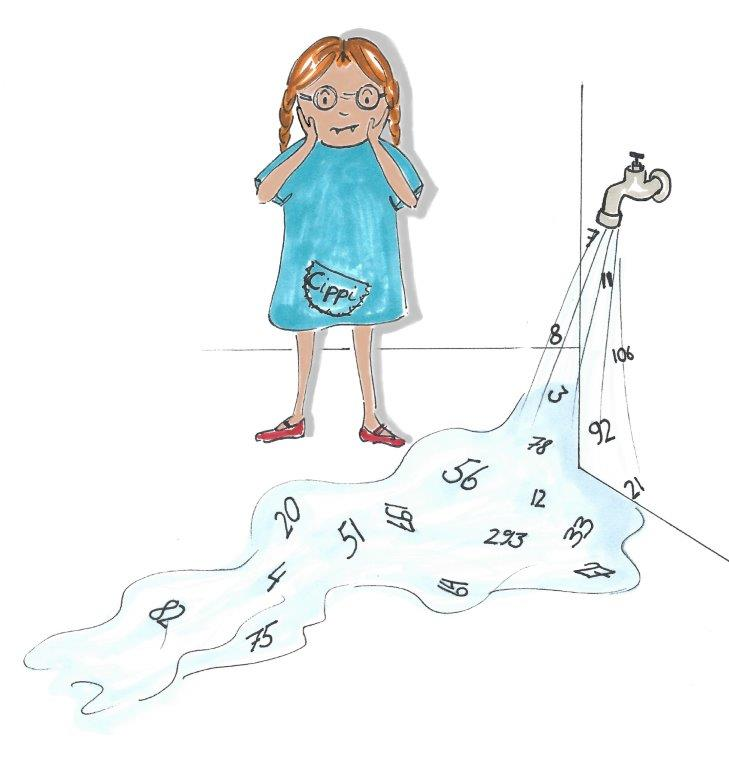
\includegraphics[width=0.8\textwidth]{content/3/chapter7/images/13.png}\\
Cippi handles a data stream
\end{center}

Before I modify and generalize the generator for an infinite data stream, I want to present it as a starting point of our journey. I intentionally put many output operations in the source code and only ask for three values. This simplification and visualization should help to understand the control flow.

\hspace*{\fill} \\ %插入空行
\noindent
Generator generating an infinite data stream
\begin{lstlisting}[style=styleCXX]
// infiniteDataStreamComments.cpp

#include <coroutine>
#include <memory>
#include <iostream>

template<typename T>
struct Generator {
	
	struct promise_type;
	using handle_type = std::coroutine_handle<promise_type>;
	
	Generator(handle_type h): coro(h) {
		std::cout << " Generator::Generator" << '\n';
	}
	handle_type coro;
	
	~Generator() {
		std::cout << " Generator::~Generator" << '\n';
		if ( coro ) coro.destroy();
	}
	Generator(const Generator&) = delete;
	Generator& operator = (const Generator&) = delete;
	Generator(Generator&& oth): coro(oth.coro) {
		oth.coro = nullptr;
	}
	Generator& operator = (Generator&& oth) {
		coro = oth.coro;
		oth.coro = nullptr;
		return *this;
	}
	int getNextValue() {
		std::cout << " Generator::getNextValue" << '\n';
		coro.resume();
		return coro.promise().current_value;
	}
	struct promise_type {
		promise_type() {
			std::cout << " promise_type::promise_type" << '\n';
		}
		
		~promise_type() {
			std::cout << " promise_type::~promise_type" << '\n';
		}
		
		std::suspend_always initial_suspend() {
			std::cout << " promise_type::initial_suspend" << '\n'; \
			
			return {};
		}
		std::suspend_always final_suspend() noexcept {
			std::cout << " promise_type::final_suspend" << '\n';
			return {};
		}
		auto get_return_object() {
			std::cout << " promise_type::get_return_object" << '\n'; \
			
			return Generator{handle_type::from_promise(*this)};
		}
		std::suspend_always yield_value(int value) {
			std::cout << " promise_type::yield_value" << '\n'; \
			
			current_value = value;
			return {};
		}
		void return_void() {}
		void unhandled_exception() {
			std::exit(1);
		}
		
		T current_value;
	};
	
};

Generator<int> getNext(int start = 10, int step = 10) {
	std::cout << " getNext: start" << '\n';
	auto value = start;
	while (true) {
		std::cout << " getNext: before co_yield" << '\n';
		co_yield value;
		std::cout << " getNext: after co_yield" << '\n';
		value += step;
	}
}

int main() {

	auto gen = getNext();
	for (int i = 0; i <= 2; ++i) {
		auto val = gen.getNextValue();
		std::cout << "main: " << val << '\n';
	}

}
\end{lstlisting}

Executing the program on the \href{https://godbolt.org/z/cTW9Gq}{Compiler Explorer} makes the control flow transparent.

\begin{center}
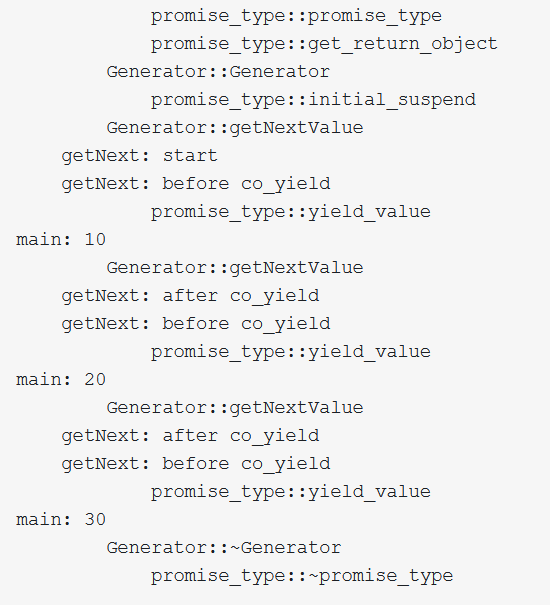
\includegraphics[width=0.8\textwidth]{content/3/chapter7/images/14.png}\\
Generator generating an infinite data stream
\end{center}

Let’s analyze the control flow.

The call getNext() (line 87) triggers the creation of the Generator<int>. First, the promise\_type (line 38) is created, and the following get\_return\_object call (line 54) creates the generator (line 56) and stores it in a local variable. The result of this call is returned to the caller when the coroutine is suspended the first time. The initial suspension happens immediately (line 48). Because the member function call initial\_suspend returns an Awaitable std::suspend\_always (line 48), the control flow continues with the coroutine getNext until the instruction co\_yield value (line 79). This call is mapped to the call yield\_value(int value) (line 59) and the current value is prepared current\_value = value (line 61). The member function yield\_value(int value) returns the Awaitable std::suspend\_always (line 59). Consequently, the execution of the coroutine pauses, and the control flow goes back to the main function, and the for loop starts (line 89). The call gen.getNextValue() (line 89) starts the execution of the coroutine by resuming the coroutine, using coro.resume() (line 34). Further, the function getNextValue() returns the current value that was prepared using the previously invoked member function yield\_value(int value) (line 59). Finally, the generated number is displayed in line 90 and the for loop continues. In the end, the generator and the promise are destructed.

After this detailed analysis, I want to make a first modification of the control flow.

\subsubsubsection{7.3.1\hspace{0.2cm} Modifications}

The snippets and line numbers are all based on the previous program infiniteDataStreamComments.cpp. I only show the modifications.

\hspace*{\fill} \\ %插入空行
\noindent
\textbf{7.3.3.1\hspace{0.2cm} The Coroutine is Not Resumed}

When I disable the resumption of the coroutine (gen.getNextValue() in line 89) and the display of its value (line 90), the coroutine immediately pauses.

\hspace*{\fill} \\ %插入空行
\noindent
Not resuming the coroutine
\begin{lstlisting}[style=styleCXX]
int main() {
	
	auto gen = getNext();
	for (int i = 0; i <= 2; ++i) {
		// auto val = gen.getNextValue();
		// std::cout << "main: " << val << '\n';
	}

}
\end{lstlisting}

The coroutine never runs. Consequently, the generator and its promise are created and destroyed.

\begin{center}
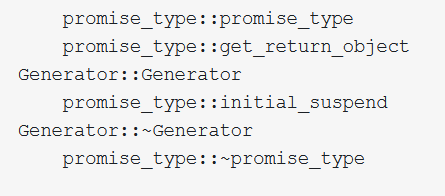
\includegraphics[width=0.8\textwidth]{content/3/chapter7/images/15.png}\\
Not resuming the coroutine
\end{center}

\hspace*{\fill} \\ %插入空行
\noindent
\textbf{7.3.3.2\hspace{0.2cm} initial\_suspend Never Suspends}

In the program, the member function initial\_suspend returns the Awaitable std::suspend\_always (line 46). As its name suggests, the Awaitable std::suspends\_always causes the coroutine to pause immediately. Let me return std::suspend\_never instead of std::suspend\_always.

\hspace*{\fill} \\ %插入空行
\noindent
initial\_suspend suspends never
\begin{lstlisting}[style=styleCXX]
std::suspend_never initial_suspend() {
	std::cout << " promise_type::initial_suspend" << '\n';
	return {};
}
\end{lstlisting}

In this case, the coroutine runs immediately and pauses when the function yield\_value (line 59) is invoked. A subsequent call gen.getNextValue() (line 89) resumes the coroutine and triggers the execution of the member function yield\_value once more. The result is that the start value 10 is ignored, and the coroutine returns the values 20, 30, and 40.

\begin{center}
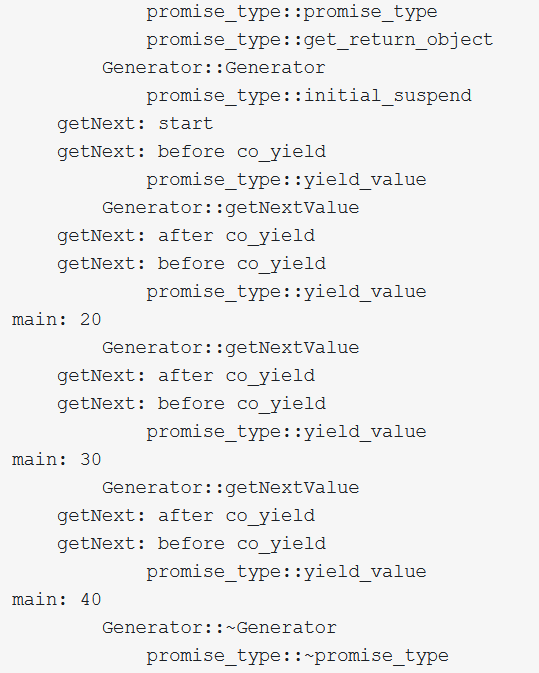
\includegraphics[width=0.8\textwidth]{content/3/chapter7/images/16.png}\\
Don’t Resuming the Coroutine
\end{center}

\hspace*{\fill} \\ %插入空行
\noindent
\textbf{7.3.3.3\hspace{0.2cm} yield\_value Never Suspends}

The member function yield\_value (line 59) is triggered by the call co\_yield value and prepares the current\_value (line 61). The function returns the Awaitable std::suspend\_always (line 62) and, therefore, pauses the coroutine. Consequently, a subsequent call gen.getNextValue (line 89) has to resume the coroutine. When I change the return value of the member function yield\_value to std::suspend\_never, let me see what happens.

\hspace*{\fill} \\ %插入空行
\noindent
yield\_value never suspends
\begin{lstlisting}[style=styleCXX]
std::suspend_never yield_value(int value) {
	std::cout << " promise_type::yield_value" << '\n';
	current_value = value;
	return {};
}
\end{lstlisting}

As you may guess, the while loop (lines 77 - 82) runs forever, and the coroutine does not return anything.

\begin{center}
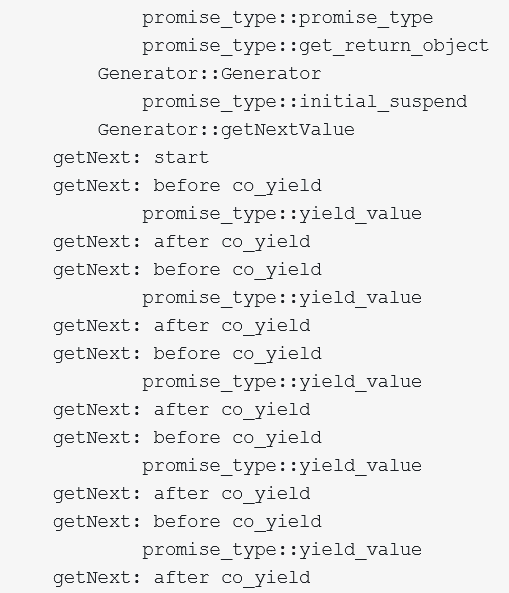
\includegraphics[width=0.8\textwidth]{content/3/chapter7/images/17.png}\\
yield\_value Never Suspends
\end{center}

It is straightforward to restructure the generator infiniteDataStreamComments.cpp so that it produces a finite number of values.

\subsubsubsection{7.3.2\hspace{0.2cm} Generalization}

You may wonder why I never used the full generic potential of Generator. Let me adjust its implementation to produce the successive elements of an arbitrary container of the Standard Template Library.

\hspace*{\fill} \\ %插入空行
\noindent
Generator successively returning each element
\begin{lstlisting}[style=styleCXX]
// coroutineGetElements.cpp

#include <coroutine>
#include <memory>
#include <iostream>
#include <string>
#include <vector>

template<typename T>
struct Generator {

	struct promise_type;
	using handle_type = std::coroutine_handle<promise_type>;
	
	Generator(handle_type h): coro(h) {}
	
	handle_type coro;
	
	~Generator() {
		if ( coro ) coro.destroy();
	}
	Generator(const Generator&) = delete;
	Generator& operator = (const Generator&) = delete;
	Generator(Generator&& oth): coro(oth.coro) {
		oth.coro = nullptr;
	}
	Generator& operator = (Generator&& oth) {
		coro = oth.coro;
		oth.coro = nullptr;
		return *this;
	}
	T getNextValue() {
		coro.resume();
		return coro.promise().current_value;
	}
	struct promise_type {
		promise_type() {}
		
		~promise_type() {}
		
		std::suspend_always initial_suspend() {
			return {};
		}
		std::suspend_always final_suspend() noexcept {
			return {};
		}
		auto get_return_object() {
			return Generator{handle_type::from_promise(*this)};
		}
		
		std::suspend_always yield_value(const T value) {
			current_value = value;
			return {};
		}
		void return_void() {}
		void unhandled_exception() {
			std::exit(1);
		}
		
		T current_value;
	};

};

template <typename Cont>
Generator<typename Cont::value_type> getNext(Cont cont) {
	for (auto c: cont) co_yield c;
}

int main() {

	std::cout << '\n';
	
	std::string helloWorld = "Hello world";
	auto gen = getNext(helloWorld);
	for (int i = 0; i < helloWorld.size(); ++i) {
		std::cout << gen.getNextValue() << " ";
	}
	
	std::cout << "\n\n";
	
	auto gen2 = getNext(helloWorld);
	for (int i = 0; i < 5 ; ++i) {
		std::cout << gen2.getNextValue() << " ";
	}
	
	std::cout << "\n\n";
	
	std::vector myVec{1, 2, 3, 4 ,5};
	auto gen3 = getNext(myVec);
	for (int i = 0; i < myVec.size() ; ++i) {
		std::cout << gen3.getNextValue() << " ";
	}
	
	std::cout << '\n';

}
\end{lstlisting}

In this example, the generator is instantiated and used three times. In the first two cases, gen (line 76) and gen2 (line 83) are initialized with std::string helloWorld, while gen3 uses a std::vector<int> (line 91). The output of the program should not be surprising. Line 78 returns all characters of the string helloWorld successively, line 85 only the first five characters, and line 93 the elements of the std::vector<int>.

You can try out the program on the \href{https://godbolt.org/z/j9znva}{Compiler Explorer}.

\begin{tcblisting}{commandshell={}}
H e l l o  w o r l d

H e l l o

1 2 3 4 5
\end{tcblisting}

\begin{center}
A generator successively returning each element
\end{center}

To make it short. The implementation of the Generator<T> is almost identical to the previous one. The crucial difference with the previous program is the coroutine getNext.

\hspace*{\fill} \\ %插入空行
\noindent
getNext
\begin{lstlisting}[style=styleCXX]
template <typename Cont>
Generator<typename Cont::value_type> getNext(Cont cont) {
	for (auto c: cont) co_yield c;
}
\end{lstlisting}

getNext is a function template that takes a container as an argument and iterates in a range-based for loop through all elements of the container. After each iteration, the function template pauses. The return type Generator<typename Cont::value\_type> may look surprising to you. Cont::value\_type is a dependent template parameter, for which the parser needs a hint. By default, the compiler assumes a non-type if it could be interpreted as a type or a non-type. For this reason, I have to put typename in front of Cont::value\_type.















